% Fibrado principal — trivialización local
% Compilar con: pdflatex fiber_bundle.tex
\documentclass[tikz,border=10pt]{standalone}
\usepackage{tikz}
\usepackage{amsmath,amssymb}
\usepackage{xcolor}
\definecolor{gdlblue}{RGB}{41, 98, 168}
\definecolor{gdlred}{RGB}{191, 49, 49}
\definecolor{gdlgreen}{RGB}{30, 130, 76}
\definecolor{gdlorange}{RGB}{217, 130, 30}
\definecolor{gdlpurple}{RGB}{118, 56, 138}
\definecolor{gdlgray}{RGB}{140, 140, 140}
\definecolor{gdlyellow}{RGB}{190, 140, 10}
\usetikzlibrary{arrows.meta, decorations.pathmorphing, calc, patterns}

\begin{document}
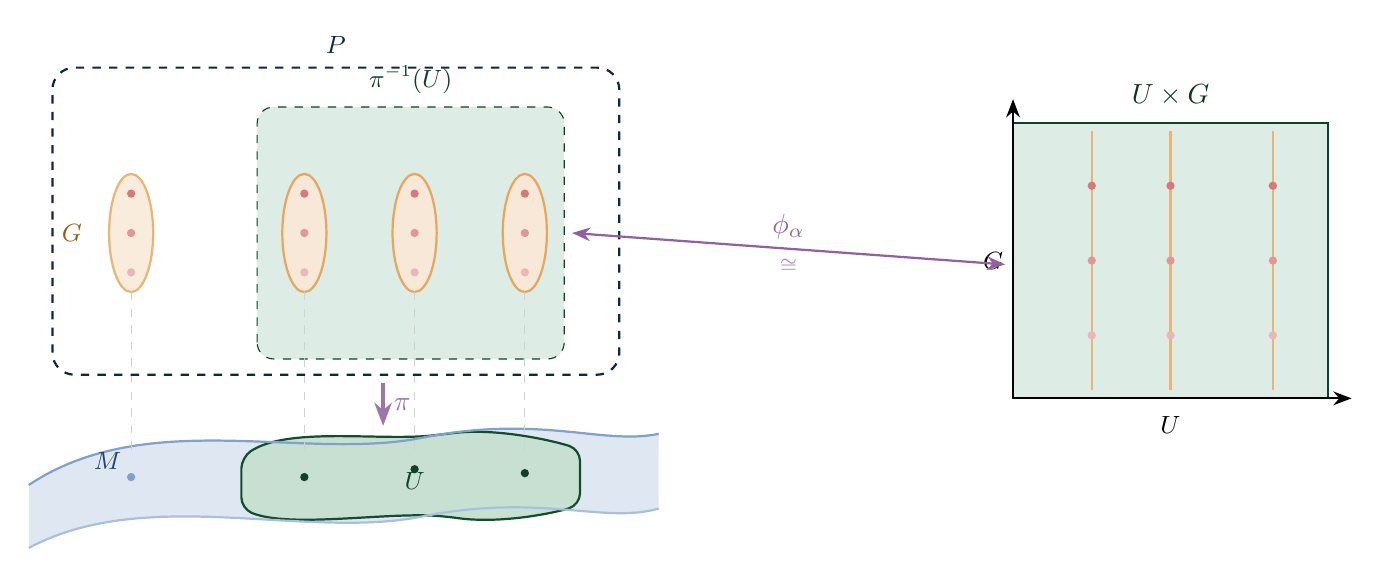
\begin{tikzpicture}[>=Stealth, font=\small]

% =====================================================
% LADO IZQUIERDO: EL FIBRADO  P → M
% =====================================================

% --- Base M (superficie curva) ---
\begin{scope}
    % Superficie completa M
    \fill[gdlblue!15]
        (-4.5, -0.6) .. controls (-3, 0.4) and (-1, -0.3) .. (0.5, 0)
        .. controls (2, 0.3) and (2.8, -0.1) .. (3.5, 0.05)
        -- (3.5, -0.9) .. controls (2.8, -1.1) and (2, -0.7) .. (0.5, -1.0)
        .. controls (-1, -1.3) and (-3, -0.6) .. (-4.5, -1.4) -- cycle;

    % Subconjunto U sombreado
    \fill[gdlgreen!25, rounded corners=4pt]
        (-1.8, -0.25) .. controls (-1.2, 0.15) and (0, -0.05) .. (0.8, 0.05)
        .. controls (1.5, 0.12) and (2.2, -0.05) .. (2.5, -0.15)
        -- (2.5, -0.85)
        .. controls (2.2, -0.95) and (1.5, -1.1) .. (0.8, -1.0)
        .. controls (0, -0.95) and (-1.2, -1.15) .. (-1.8, -0.9)
        -- cycle;
    \draw[gdlgreen!60!black, thick, rounded corners=4pt]
        (-1.8, -0.25) .. controls (-1.2, 0.15) and (0, -0.05) .. (0.8, 0.05)
        .. controls (1.5, 0.12) and (2.2, -0.05) .. (2.5, -0.15)
        -- (2.5, -0.85)
        .. controls (2.2, -0.95) and (1.5, -1.1) .. (0.8, -1.0)
        .. controls (0, -0.95) and (-1.2, -1.15) .. (-1.8, -0.9)
        -- cycle;

    % Borde superior de M
    \draw[thick, gdlblue!60]
        (-4.5, -0.6) .. controls (-3, 0.4) and (-1, -0.3) .. (0.5, 0)
        .. controls (2, 0.3) and (2.8, -0.1) .. (3.5, 0.05);
    % Borde inferior de M
    \draw[thick, gdlblue!40]
        (-4.5, -1.4) .. controls (-3, -0.6) and (-1, -1.3) .. (0.5, -1.0)
        .. controls (2, -0.7) and (2.8, -1.1) .. (3.5, -0.9);

    % Etiquetas base
    \node[gdlblue!70!black] at (-3.5, -0.3) {$M$};
    \node[gdlgreen!50!black] at (0.4, -0.55) {$U$};

    % Puntos en U
    \coordinate (p1) at (-1.0, -0.5);
    \coordinate (p2) at (0.4, -0.4);
    \coordinate (p3) at (1.8, -0.45);
    \foreach \p in {p1, p2, p3} {
        \fill[gdlgreen!50!black] (\p) circle (1.5pt);
    }

    % Punto fuera de U (solo izquierda)
    \fill[gdlblue!60] (-3.2, -0.5) circle (1.5pt);
\end{scope}

% --- Espacio total P (arriba) ---
\begin{scope}

    % Sombreado suave para π⁻¹(U) agrupando fibras sobre U
    \fill[gdlgreen!15, rounded corners=6pt]
        (-1.6, 1.0) rectangle (2.3, 4.2);
    \draw[gdlgreen!50!black, dashed, rounded corners=6pt]
        (-1.6, 1.0) rectangle (2.3, 4.2);
    \node[gdlgreen!50!black, anchor=south] at (0.35, 4.25) {$\pi^{-1}(U)$};

    % Fibras como elipses verticales (grupo G)
    % Fibra fuera de U (solo a la izquierda, para no obstruir φ_α)
    \draw[thick, gdlorange!60, fill=gdlorange!15]
        (-3.2, 2.6) ellipse (0.28cm and 0.75cm);
    \fill[gdlred!65] (-3.2, 3.1) circle (1.5pt);
    \fill[gdlred!50] (-3.2, 2.6) circle (1.5pt);
    \fill[gdlred!35] (-3.2, 2.1) circle (1.5pt);
    \draw[gdlgray!40, dashed] (-3.2, 1.85) -- (-3.2, -0.2);

    % Fibras sobre U (dentro de π⁻¹(U))
    \foreach \xpos in {-1.0, 0.4, 1.8} {
        \draw[thick, gdlorange!70, fill=gdlorange!18]
            (\xpos, 2.6) ellipse (0.28cm and 0.75cm);
        \fill[gdlred!65] (\xpos, 3.1) circle (1.5pt);
        \fill[gdlred!50] (\xpos, 2.6) circle (1.5pt);
        \fill[gdlred!35] (\xpos, 2.1) circle (1.5pt);
        % Líneas de conexión a base
        \draw[gdlgray!40, dashed] (\xpos, 1.85) -- (\xpos, -0.2);
    }

    % Contorno del espacio total P
    \draw[thick, gdlblue!40!black, rounded corners=8pt, dashed]
        (-4.2, 0.8) rectangle (3.0, 4.7);
    \node[gdlblue!40!black, anchor=south] at (-0.6, 4.75) {$P$};

    % Etiqueta de fibra G (junto a la fibra fuera de U)
    \node[gdlorange!70!black, left] at (-3.7, 2.6) {$G$};
\end{scope}

% --- Proyección π ---
\draw[->, very thick, gdlpurple!70]
    (0, 0.7) -- node[right, font=\normalsize] {$\pi$} (0, 0.15);

% =====================================================
% LADO DERECHO: EL PRODUCTO  U × G
% =====================================================

\begin{scope}[shift={(9.5, 0.5)}]

    % Rectángulo U × G
    \fill[gdlgreen!15] (-1.5, 0) rectangle (2.5, 3.5);
    \draw[thick, gdlgreen!50!black] (-1.5, 0) rectangle (2.5, 3.5);

    % Eje horizontal (U)
    \draw[->, thick] (-1.5, 0) -- (2.8, 0);
    \node[below] at (0.5, -0.1) {$U$};

    % Eje vertical (G)
    \draw[->, thick] (-1.5, 0) -- (-1.5, 3.8);
    \node[left] at (-1.5, 1.75) {$G$};

    % Etiqueta producto
    \node[gdlgreen!40!black, font=\normalsize] at (0.5, 3.85) {$U \times G$};

    % Columnas de puntos (fibras trivializadas)
    \foreach \xpos/\label in {-0.5/x_1, 0.5/x_2, 1.8/x_3} {
        \draw[gdlorange!60, thick] (\xpos, 0.1) -- (\xpos, 3.4);
        \fill[gdlred!65] (\xpos, 2.7) circle (1.5pt);
        \fill[gdlred!50] (\xpos, 1.75) circle (1.5pt);
        \fill[gdlred!35] (\xpos, 0.8) circle (1.5pt);
    }
\end{scope}

% =====================================================
% CONEXIÓN: difeomorfismo φ_α
% =====================================================

\draw[<->, thick, gdlpurple!80]
    (2.4, 2.6) -- node[above, font=\normalsize] {$\phi_\alpha$}
    node[below, font=\scriptsize, gdlpurple!60] {$\cong$} (7.9, 2.2);

\end{tikzpicture}
\end{document}
